% USEFUL LINKS:
% -------------
%
% - UiO LaTeX guides:          https://www.mn.uio.no/ifi/tjenester/it/hjelp/latex/
% - Mathematics:               https://en.wikibooks.org/wiki/LaTeX/Mathematics
% - Physics:                   https://ctan.uib.no/macros/latex/contrib/physics/physics.pdf
% - Basics of Tikz:            https://en.wikibooks.org/wiki/LaTeX/PGF/Tikz
% - All the colors!            https://en.wikibooks.org/wiki/LaTeX/Colors
% - How to make tables:        https://en.wikibooks.org/wiki/LaTeX/Tables
% - Code listing styles:       https://en.wikibooks.org/wiki/LaTeX/Source_Code_Listings
% - \includegraphics           https://en.wikibooks.org/wiki/LaTeX/Importing_Graphics
% - Learn more about figures:  https://en.wikibooks.org/wiki/LaTeX/Floats,_Figures_and_Captions
% - Automagic bibliography:    https://en.wikibooks.org/wiki/LaTeX/Bibliography_Management  (this one is kinda difficult the first time)
%
%                              (This document is of class "revtex4-1", the REVTeX Guide explains how the class works)
%   REVTeX Guide:              http://www.physics.csbsju.edu/370/papers/Journal_Style_Manuals/auguide4-1.pdf
%
%
% COMPILING THE .pdf FILE IN THE LINUX TERMINAL
% ---------------------------------------------
%
% [terminal]$ pdflatex report_example.tex
%
% Run the command twice, always.
%
% When using references, footnotes, etc. you should run the following chain of commands:
%
% [terminal]$ pdflatex report_example.tex
% [terminal]$ bibtex report_example
% [terminal]$ pdflatex report_example.tex
% [terminal]$ pdflatex report_example.tex
%
% This series of commands can of course be gathered into a single-line command:
% [terminal]$ pdflatex report_example.tex && bibtex report_example.aux && pdflatex report_example.tex && pdflatex report_example.tex
%
% ----------------------------------------------------



\documentclass[english,notitlepage,reprint,nofootinbib]{revtex4-1}  % defines the basic parameters of the document
% If you want a single-column, remove "reprint"

% Allows special characters (including æøå)
\usepackage[utf8]{inputenc}
% \usepackage[english]{babel}

% Note that you may need to download some of these packages manually, it depends on your setup.
% It may be usefult to download TeXMaker, because it includes a large library of the most common packages.

\usepackage{physics,amssymb}  % mathematical symbols (physics imports amsmath)
\include{amsmath}
\usepackage{graphicx}         % include graphics such as plots
\usepackage{xcolor}           % set colors
\usepackage{hyperref}         % automagic cross-referencing
\usepackage{listings}         % display code
\usepackage{subfigure}        % imports a lot of cool and useful figure commands
% \usepackage{float}
%\usepackage[section]{placeins}
\usepackage{algorithm}
\usepackage[noend]{algpseudocode}
\usepackage{subfigure}
\usepackage{comment}
\usepackage{placeins}
\usepackage{tikz}
\usetikzlibrary{quantikz}
% defines the color of hyperref objects
% Blending two colors:  blue!80!black  =  80% blue and 20% black
\hypersetup{ % this is just my personal choice, feel free to change things
    colorlinks,
    linkcolor={red!50!black},
    citecolor={blue!50!black},
    urlcolor={blue!80!black}}


% ===========================================


\begin{document}

\title{Wavefunction interferance}  % self-explanatory
\author{Lukas Cernusak} % self-explanatory
\date{December 2023}                             % self-explanatory
\noaffiliation                            % ignore this, but keep it.




%This is how we create an abstract section.
\begin{abstract}
We simulate the behavior of a dimensionless quantum wavefunction in 2D, for both single, double, and triple slits. The boundary values are zero, which corresponds to the system being enclosed in an infinite square well. The initial wavefunction is a wavepocket in the form of natural exponential. The algorithm that's used is the Crank-Nicolson scheme, in matrix form. There are plots with probability densities, both real and imaginary parts of the wavefunction, detection probability, and normalization for different times. We validate the approach and find reasonable interference patterns. We find division from normalization on the order of $10^{-7}$, which is deemed almost suspiciously small. 
\end{abstract}
\maketitle



% ===========================================
\section{Introduction}
In the world of physics, quantum mechanics may be the single most influential theory of the last few centuries. It has changed our view of the physical world so much, that philosophical questions about its interpretations are still quite active, with the last successful theory, namely QBism $^{\text{[2]}}$, dating to 2010. In this report, we will be working with the equation governing all of non-relativistic quantum physics, namely \textit{Schrodinger equation} (SE), and studying how it predicts the behavior in may be the best-known experiment of them all, the slit experiment.

Quantum mechanics, models particles as a superposition of waves rotating in a complex plain. This introduces many new possibilities, compared to classical mechanics, for instance, the waves can interfere both with themselves and other waves. Therefore the slit experiments serve as a fantastic validation for the theory.

The Schrodinger equation is a \textit{particular differential equation} (PDE). Furthermore, it is a parabolic equation, meaning its future state can be determined, by knowing the past of all spatial points. This of course contradicts the special theory of relativity, which would require a function governing the Quantum to have a light-cone, meaning the equation would need to be hyperbolic.

Whether a system, described by SE, has an analytical solution boils down to its potential function. However, solving such an equation, and even finding all solutions, are generally hard work, often requiring assumptions. In this report, we will therefore solve the SE numerically, using \textit{Crank-Nicolson scheme} (CNS). The different approaches for solving PDEs numerically depend on the approximation method of individual derivatives. In the case of CNS, it uses a linear combination of forward difference and backward difference.







% ===========================================
\section{Methods}

\subsection{Physics}

The SE connects the time evolution of the quantum state to the total energy of the system. This is generally expressed as
$$ i \hbar \frac{\partial}{\partial t} \ket{\Psi} = \hat{H} \ket{\Psi} .$$

Here the $\hat{H}$ is the Hamiltonian operator and may be defined using momentum and position operators. Here the position operators are $\hat{x} = x$ and $\hat{y} = y$ just as the potential is $\hat{V} = V$. However, the momentum operator is 
$$\hat{p} =  -i \hbar \Big( \frac{\partial}{\partial x} + \frac{\partial}{\partial y} \Big),$$
such that the Hamiltonian can be defined in the usual way as 
$$\hat{H} = \frac{\hat{p} ^2}{2m} + V(x,y). $$

Furthermore, $\hbar$ is the reduced Planck's constant, and $\ket{\Psi}$ is the quantum state. To get a PDE, we will make the quantum state, the wave function $\Psi(x,y,t)$.
\begin{equation}
    i \hbar \frac{\partial}{\partial t} \Psi (x,y,t) = - \frac{\hbar ^2}{2m} \Big( \frac{\partial ^2}{\partial x^2} + \frac{\partial ^2}{\partial y^2} \Big) \Psi(x,y,t) .
\end{equation}
The $m$ corresponds to the mass of the object. Here we assume the potential $V$ is time-independant. The Planc's constant, and often also the mass, are very small. However, as we are not interested in describing any particular physical system, but rather seeing how do wavefunction behaves, we will assume the variables to be dimensionless, such that we will be solving the equation
\begin{equation} \label{eq:2}
    i \frac{\partial u}{\partial t} = - \frac{\partial ^2 u}{\partial x^2} - \frac{\partial ^2 u}{\partial y^2} + v(x,y) u .
\end{equation}
To make it obvious whether we are working with the actual wavefunction and potential or the ones in the dimensionless equation, we use a different name for them, such that $\Psi \rightarrow u$ and $V(x,y) \rightarrow v(x,y)$.

The wavefunction tells us all there is to know about the quantum system, however, all we are interested in is the probability of finding a particle in a particular position and time. As both time and space are continuum, the theory provides a probability density, defined as the absolute value squared of the wavefunction, which for the dimensionless becomes
\begin{equation}
    P(x \in [x,x+h],y \in [y, y+h];t) = u(x,y,t) u(x,y,t)^* h^2
\end{equation}
Here it becomes clear the wavefunction needs to be normalized such that the total probability adds up to one. It is in some cases possible to outrule some states as unphysical if it is not possible to normalize the wavefunction. Due to the numerical approach in this report, we will describe the normalization in detail in the following section about discretization. It is possible to prove analytically that the wave function does maintain its normalization, such that the function only needs to be normalized once. We will use this fact to validate our approach.



\subsection{Algorythms}

The simulation will be in 2+1 dimensions. The room is composed of $x$ and $y$ coordinate with definition, both with domain in the interval $D_f=[0,1]$. The boundary points, meaning all the points where $x$ or $y$ are $0$ or $1$, will be set to zero. This assumption would physically correspond to the slit, and the particle, being trapped in an infinite square well. The number of points along each axis is equal and denoted by $M$, meaning we have $M-2$ points between two boundary points. The step in the room, between two points is $h$. This means that that the positions $x$ and $y$ will be
$$ x_i = i h \quad i=0,1,\cdot \cdot \cdot, M-1$$
$$ y_j = j h \quad j=0,1,\cdot \cdot \cdot, M-1.$$
The time domain interval will be $[0,T]$, where $T$ is to be specified later. The timestep is denoted by $\Delta t$. There is a requirement for the relation between $h$ and $\Delta t$ for the stability of CNS, so $\Delta t$ will be much smaller than $h$. Similarly as with room position, the time will be denoted as
$$ t_n = n \Delta t \quad n=0,1,\cdot \cdot \cdot, \frac{T}{dt}.$$
Here it is assumed $\frac{T}{dt}$ is an integer. Combining this notation, we get the discretized wavefunction $u$ and potential $v$ will be denoted as 
$$ u_{ij}^n = u(x_i, y_j, t_n) $$
$$ v_{ij} = v(x_i, y_j). $$
As we will be evolving the state using a matrix equation, we will need to transform the matrix $u$ into a vector. The vector $\vec{u}$ is defined as
\begin{equation}
    \vec{u} = (u_{1,1},u_{1,2},\cdot \cdot \cdot, u_{1,M-2}, u_{2,1}, \cdot \cdot \cdot, u_{M-1,M-1})^T.
\end{equation}
Note that the vector doesn't include the boundary points. This vector has therefore elements $(M-2)^2$, which will be donted using a index $k$. 


The SE is a parabolic PDE, and we will use the Crank Nicolson Scheme to evolve it. The approach is explained in somewhat greater detail in Appendix A. It can be shown that the CNS can be applied by finding two matrices $A$ and $B$, where the solution for next time $t_{n+1}$ can be found as the matrix equation, with matrix $B$ and vector found by multiplying the matrix $A$ with the solution at time $t_n$, meaning
\begin{equation}
    A \vec{u}^{n+1} = B \vec{u}^n.
\end{equation}
The matricies $A$ and $B$ has the size $(M-2)^2x(M-2)^2$ and are composed of $(M-2)$ sub-metricies with size of $(M-2)x(M-2)$. The sub-metrics along the diagonal will be tridiagonal. Along the diagonal, for  $A$, they will have entries determined by
\begin{equation}
    a_k = 1 + 4r + \frac{i \Delta t}{2} v_ij
\end{equation}
and outside of the diagonal, the values will equal to $r$. Similarly for matrix $B$, along the diagonal, the values will be
\begin{equation}
    b_k = 1 - 4r - \frac{i \Delta t}{2} v_ij
\end{equation}
and outside of the diagonal, the tridiagonal sub-metrics at the diagonal will have values $-r$. The only other non-zero sub-matrices, for both $A$ and $B$ will be the ones neighboring the diagonal matrices. These will themself be diagonal matrices, with entries $r$ for $A$ and $-r$ for $B$.


We will need to choose a normalized initial state for the $u$. Here we choose the wavepacket on the form
\begin{equation}
    u(x,y,t=0) = e^{\frac{-(x-x_c)^2}{2 \sigma_x^2} - \frac{(y-y_c)^2}{2 \sigma_y^2} + ip_xx + ip_yy}
\end{equation}
Here $x_c$ and $y_c$ correspond to the positions of the maxima of the wavepacket, $\sigma_x$, and $\sigma_y$ are the standard deviations, and $p_x$ together with $p_y$ are the momentums along their respective axis. All of the values will be specified later. Note that this equation isn't normalized, and will be normalized numerically in the code. Due to our discretization, the normalization condition is
\begin{equation}
    1 = \sum_{ij} u^{0*}_{ij} u^0_{ij}
\end{equation}

We will use both single, double, and triple slit in the simulations. In all cases, the wall will be located in the center of the x-axis, with a thickness of $0.02$. The wall will be symmetrical around the y-axis with a length of the slits of $0.05$ and in the case of double and triple slits, the wall-piece separating the slits will too be $0.05$. 




\subsection{Tools}
All of the matrices and vectors in the simulation are objects made using armadillo liberty. The potential matrix $v$ is the standard matrix object, the wavefunction on the matrix form $u$ is a complex matrix, and the matrices $A$ and $B$ are sp metrics, as they are much bigger, and contain mostly zeros. For solving the matrix equation, we use inbuild armadillos to solve function for sp metrics. All complex numbers in the code are made using an armadillo. All plots are made using matplotlib, in cooperation with numpy. 





\section{Results and discussion}\label{sec:results_and_discussion}

First of all, we wish to validate our approach. As mentioned, the normalization of the wavefunction would in an analytical situation be maintained over time. Due to the numerical approach, we expect a slight deviation. There are two simulations, first without a barrier and second with the double slit. The plot of the normalization stability for both simulations is visualized in Figure \ref{fig:1}.

\begin{figure}[h!]
    \centering %Centers the figure
    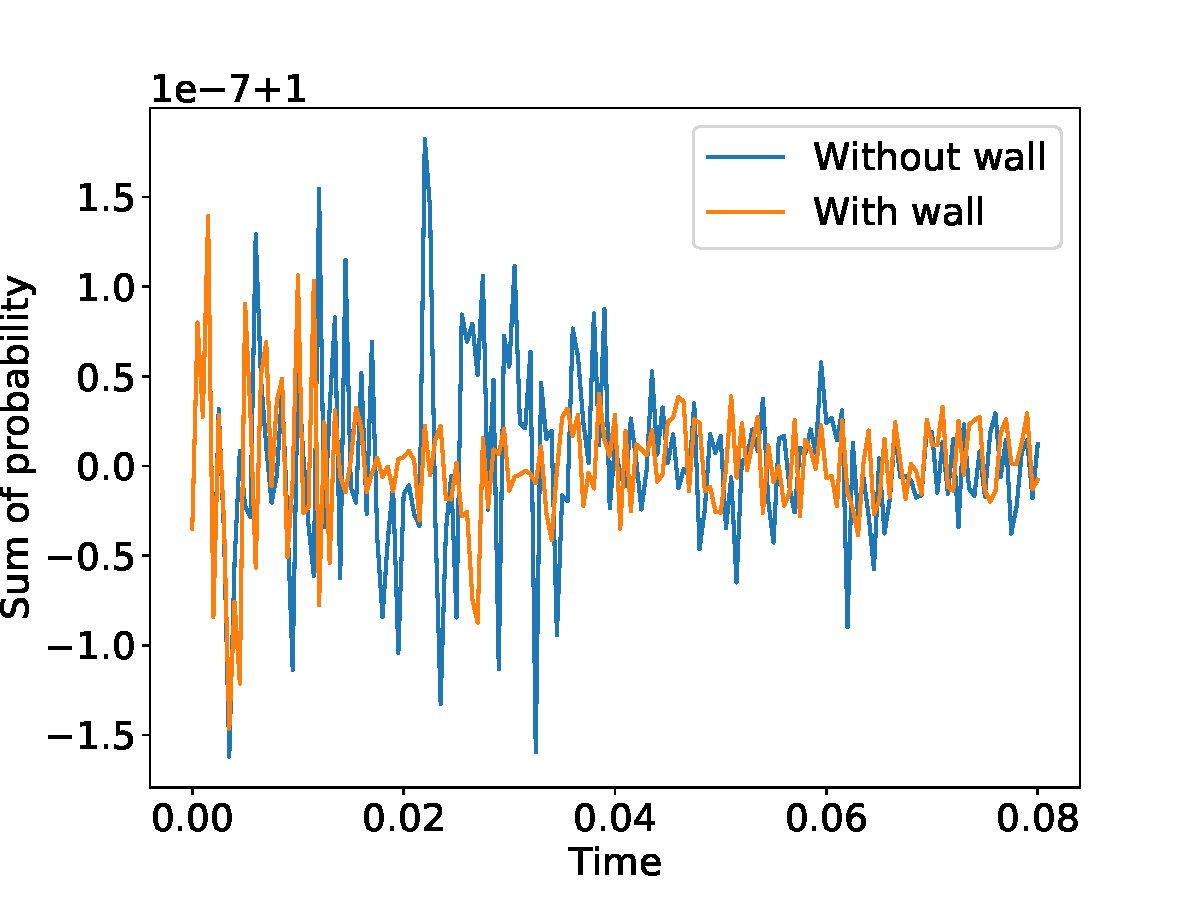
\includegraphics[scale=0.4]{figures/normlization_error.pdf} %Imports the figure.
    \caption{Plot showing how the simulation maintains normalization. The zero on the y-axis represents 1, and the axis is scaled with $10^{-7}$. The simulation had the following values: $h=0.005$, $\Delta t = 2.5\cdot 10^-5$, the potential inside the wall $v0 = 10^5$ and $0$ outside it, $x_C = 0.25$, $y_C = 0.5$, $\sigma _x = 0.05$, $p_x = 200$, $p_y = 0$ and $T = 0.008$.}
    \label{fig:1}
\end{figure}

The plots do deviate more at the beginning than at the end, for which we don't have an explanation. The deviation doesn't seem to be dependent on whether there is or isn't a barrier. The order of the deviations is very small ($10^{-7}$). From the graph, we can see that neither of the two simulations seems to start at precisely $1$, which is possibly caused by the binary representation of the floats. However, this means that the error is on the same order as the binary representation error. We don't have any expectations regarding the error, but from experience, this seems low, and it would be nice to look closer at this.

Next, we wish to visualize the wavefunction. We ran a simulation, similar to the previous one with a double slit, and we visualized the wavefunction in the room. At time zero we expect to see a wavepacket, later we expect to see the wavefunction penetrate the slits, and finally create a interference pattern after it has passed. It is also expected that part of the wavefunction will be reflected. In the Figures \ref{fig:2}, \ref{fig:3} and \ref{fig:4}, we see the probability density at three different times.

\FloatBarrier
\begin{figure}[h!]
    \centering %Centers the figure
    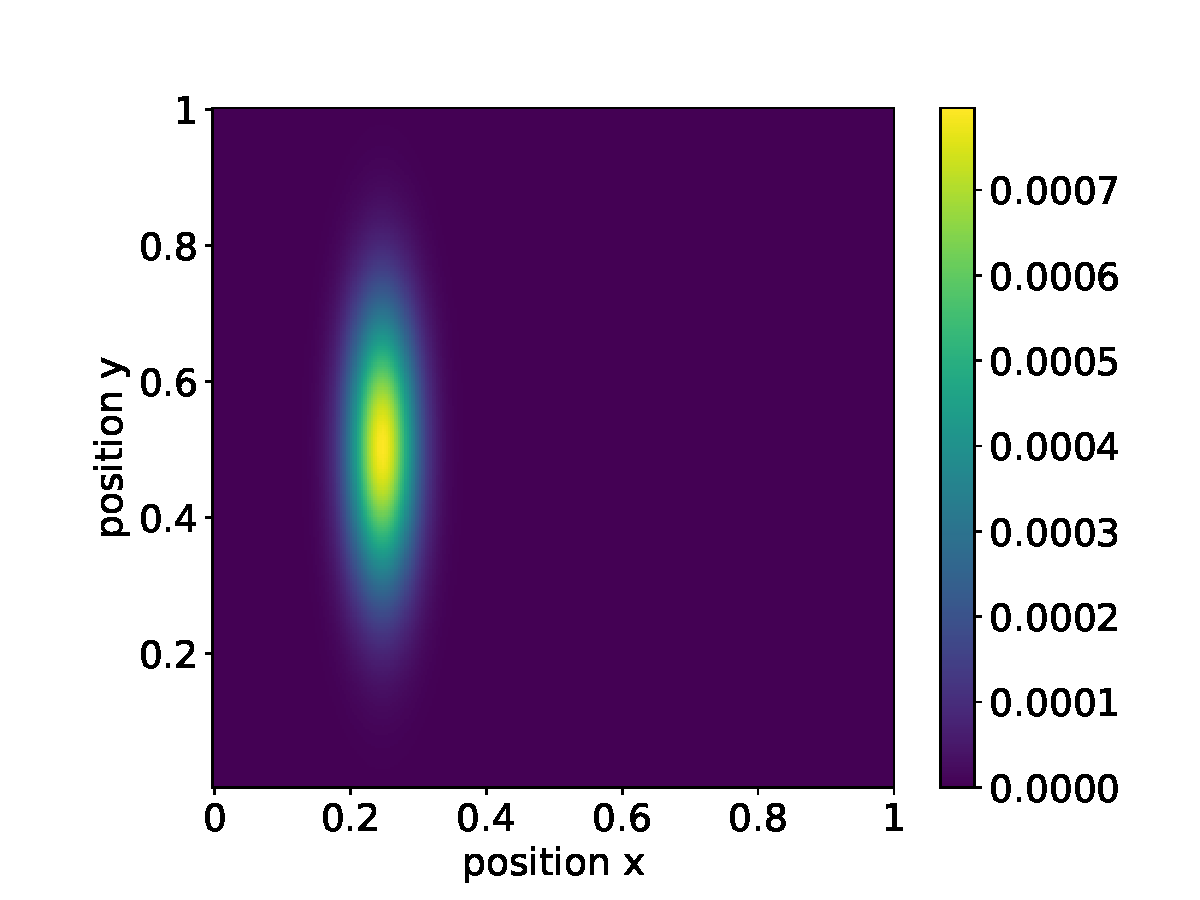
\includegraphics[scale=0.37]{figures/contur_P_2_t0.pdf} %Imports the figure.
    \caption{Plot shows the probability density of the initial wavefunction, in the form of probability mass function. The simulation had the following values: $h=0.005$, $\Delta t = 2.5\cdot 10^-5$, the potential inside the wall $v0 = 10^5$ and $0$ outside it, $x_C = 0.25$, $y_C = 0.5$, $\sigma _x = 0.05$, $\sigma _y = 0.2$, $p_x = 200$, $p_y = 0$ and $T = 0.002$.}
    \label{fig:2}
\end{figure}
\FloatBarrier

\begin{figure}[h!]
    \centering %Centers the figure
    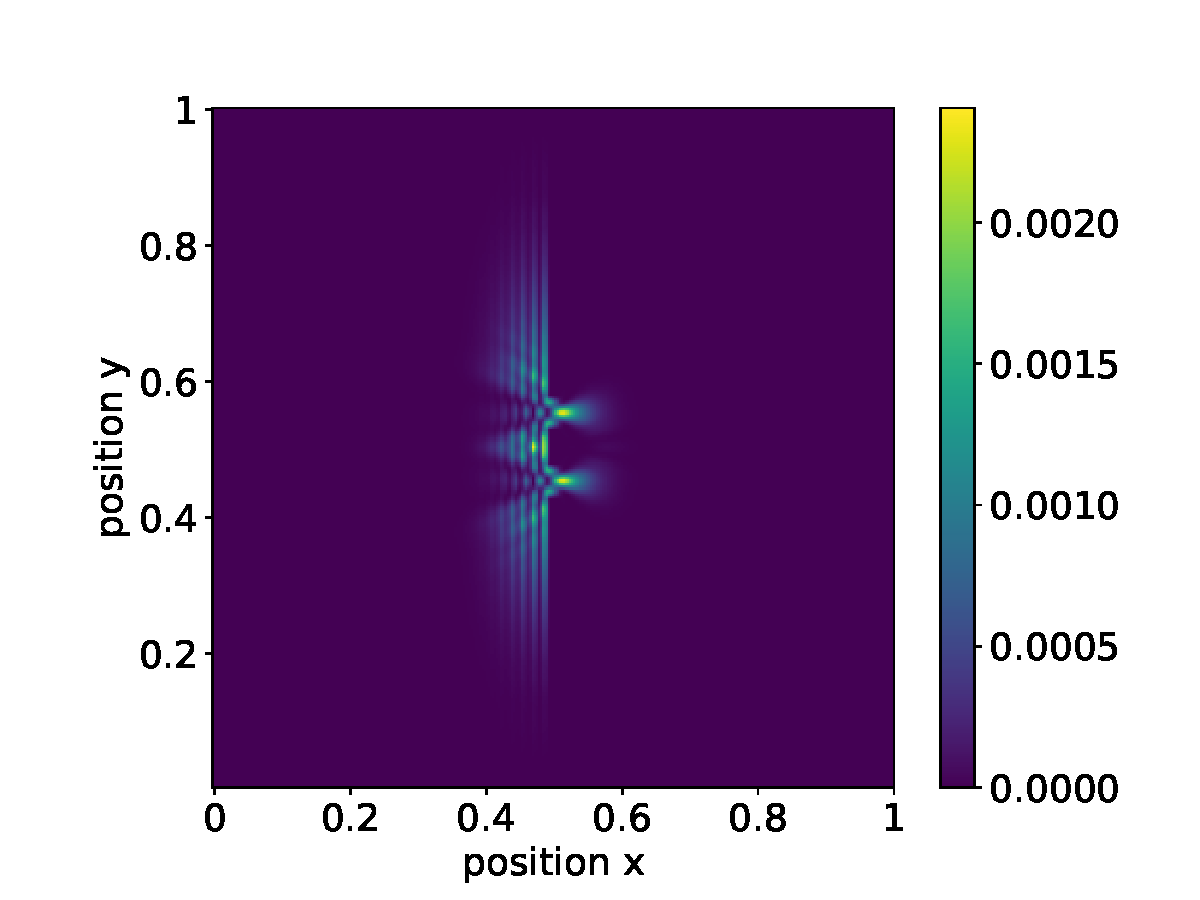
\includegraphics[scale=0.37]{figures/contur_P_2_12T.pdf} %Imports the figure.
    \caption{Plot shows the probability density at a time $t=0.001$, in the form of probability mass function. The simulation is identical to the one in figure \ref{fig:2}.}
    \label{fig:3}
\end{figure}
\FloatBarrier

There are no unexpected anomalies in the results. The choice to use probability density, while having such a small room step ($0.005$) might not have been ideal, as we are getting very low values (max $0.002$). Probability density would have worked better here.


\begin{figure}[h!]
    \centering %Centers the figure
    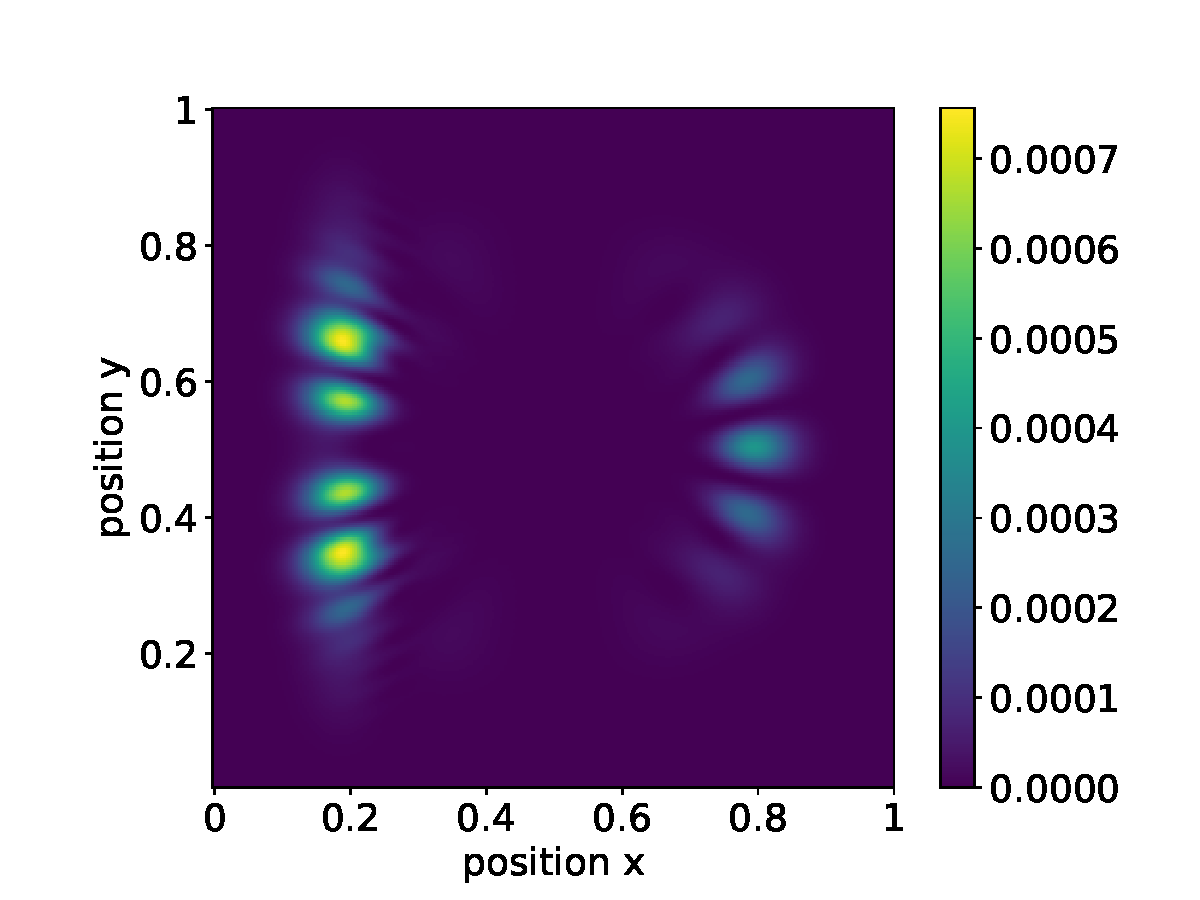
\includegraphics[scale=0.4]{figures/contur_P_2_T.pdf} %Imports the figure.
    \caption{Plot shows the probability density at a time $t=0.002$, in the form of probability mass function. The simulation is identical to the one in figure \ref{fig:2}.}
    \label{fig:4}
\end{figure}
\FloatBarrier


It might also be interesting to visualize the imaginary and real parts of the wavefunction separately. It is hard to predict how such plots will behave in the future, but we know that the initial wavefunction is specified such that there should be ripples along the x-axis, which should be phase shifted by $\frac{\pi}{2}$ relative to each other. This was specified by the momentum in the initial state. Figure \ref{fig:5} to \ref{fig:7} visualizes the real parts and figures \ref{fig:8} to \ref{fig:10} the imaginary parts.


\begin{figure}[h!]
    \centering %Centers the figure
    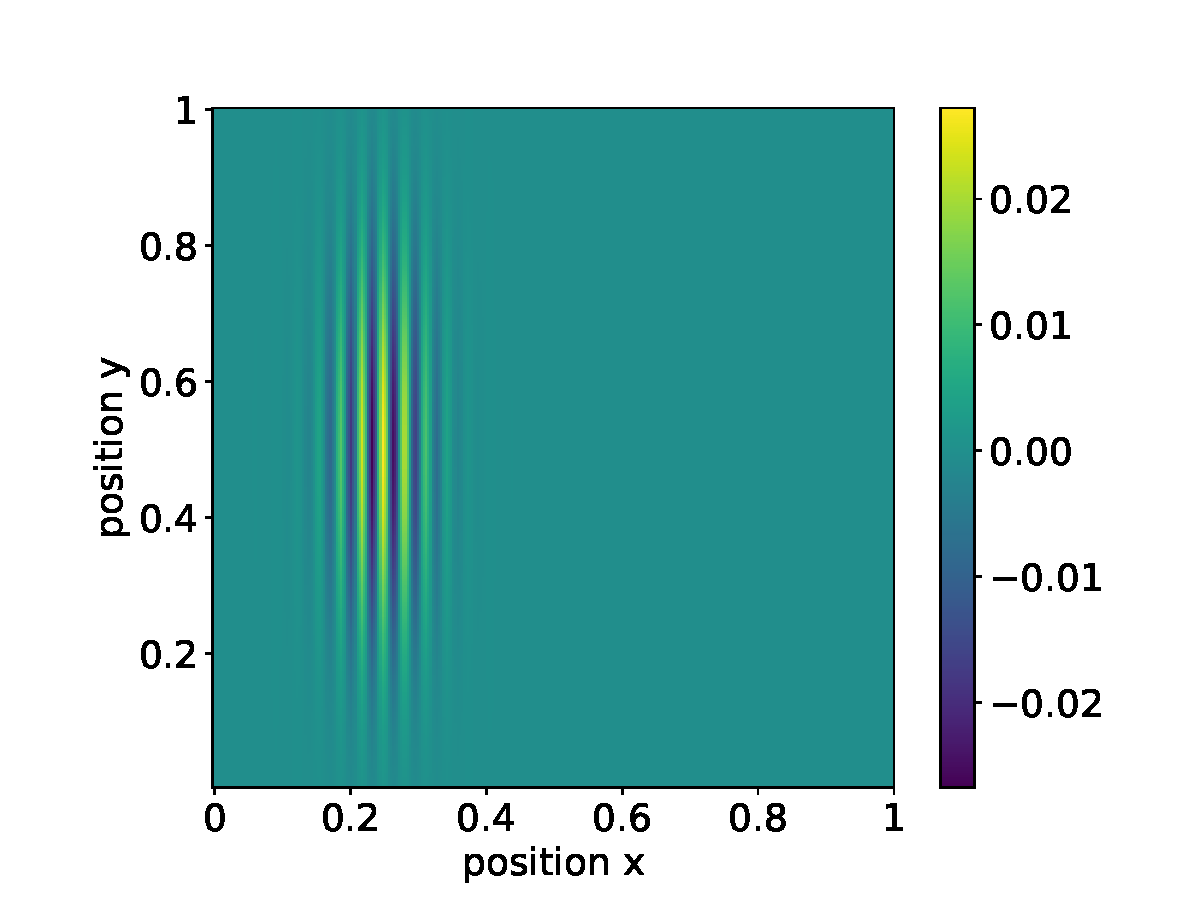
\includegraphics[scale=0.35]{figures/contur_rel_2_t0.pdf} %Imports the figure.
    \caption{Plot showing the real part of the wavefunction at a time $t=0$. The simulation is identical to the one in figure \ref{fig:2}.}
    \label{fig:5}
\end{figure}
\FloatBarrier

\begin{figure}[h!]
    \centering %Centers the figure
    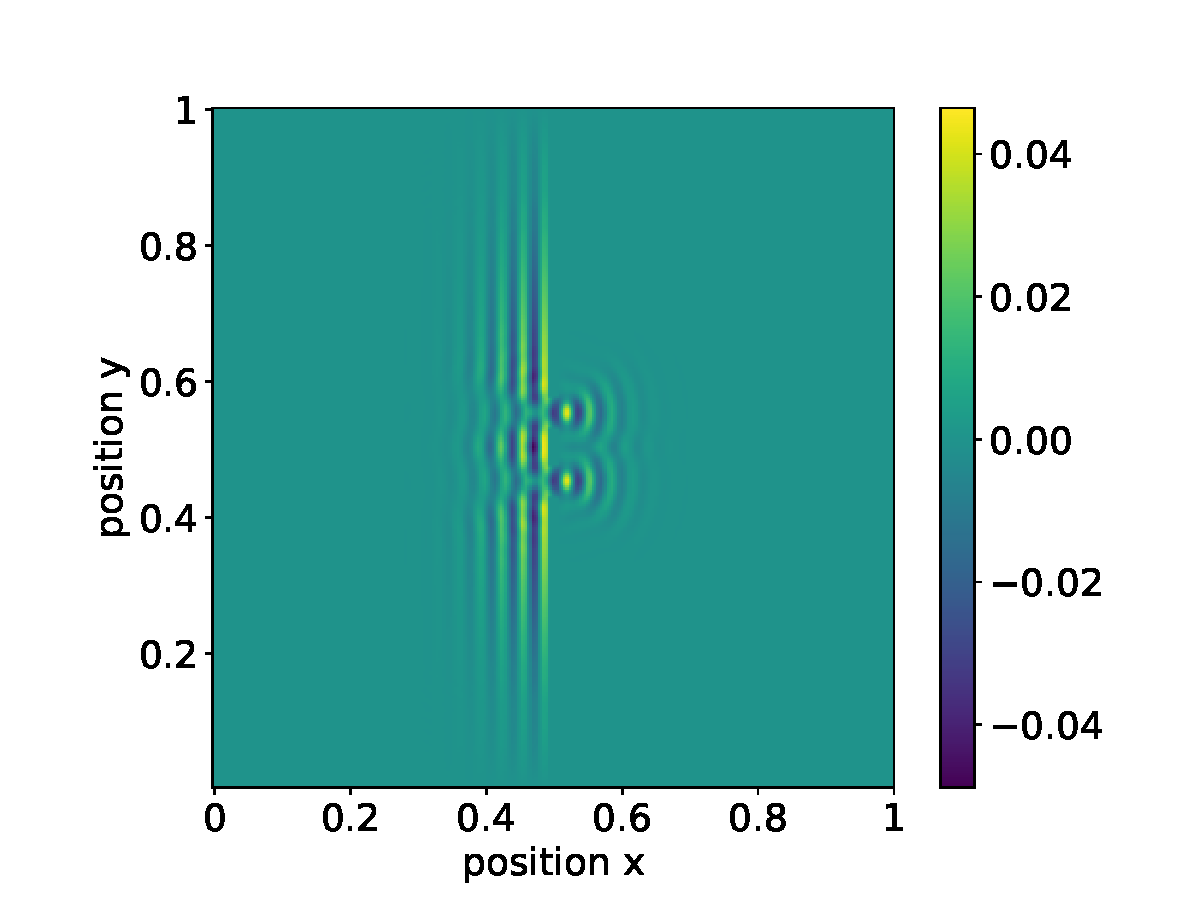
\includegraphics[scale=0.35]{figures/contur_rel_2_12T.pdf} %Imports the figure.
    \caption{Plot showing the real part of the wavefunction at a time $t=0.001$. The simulation is identical to the one in figure \ref{fig:2}.}
    \label{fig:6}
\end{figure}
\FloatBarrier



\begin{figure}[h!]
    \centering %Centers the figure
    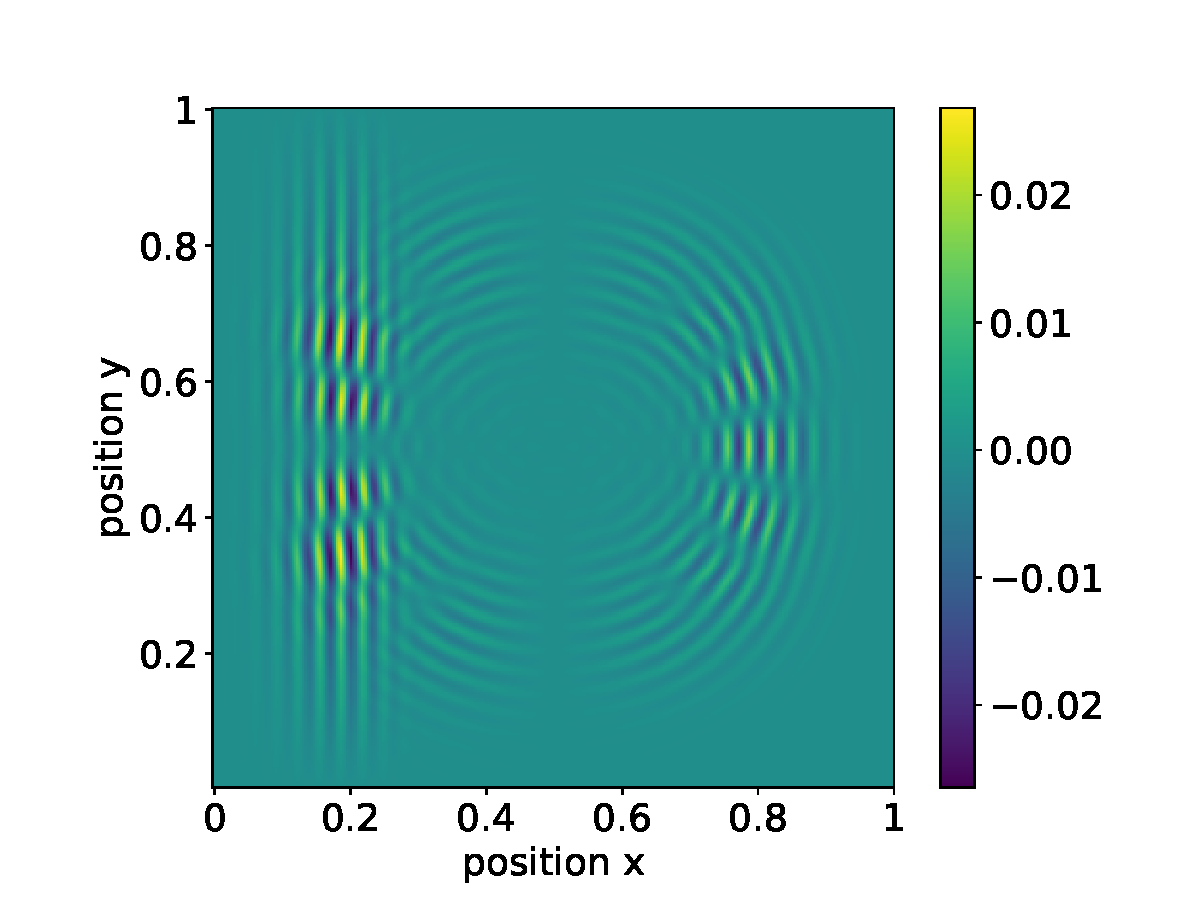
\includegraphics[scale=0.35]{figures/contur_rel_2_T.pdf} %Imports the figure.
    \caption{Plot showing the real part of the wavefunction at a time $t=0.002$. The simulation is identical to the one in figure \ref{fig:2}.}
    \label{fig:7}
\end{figure}
\FloatBarrier


\begin{figure}[h!]
    \centering %Centers the figure
    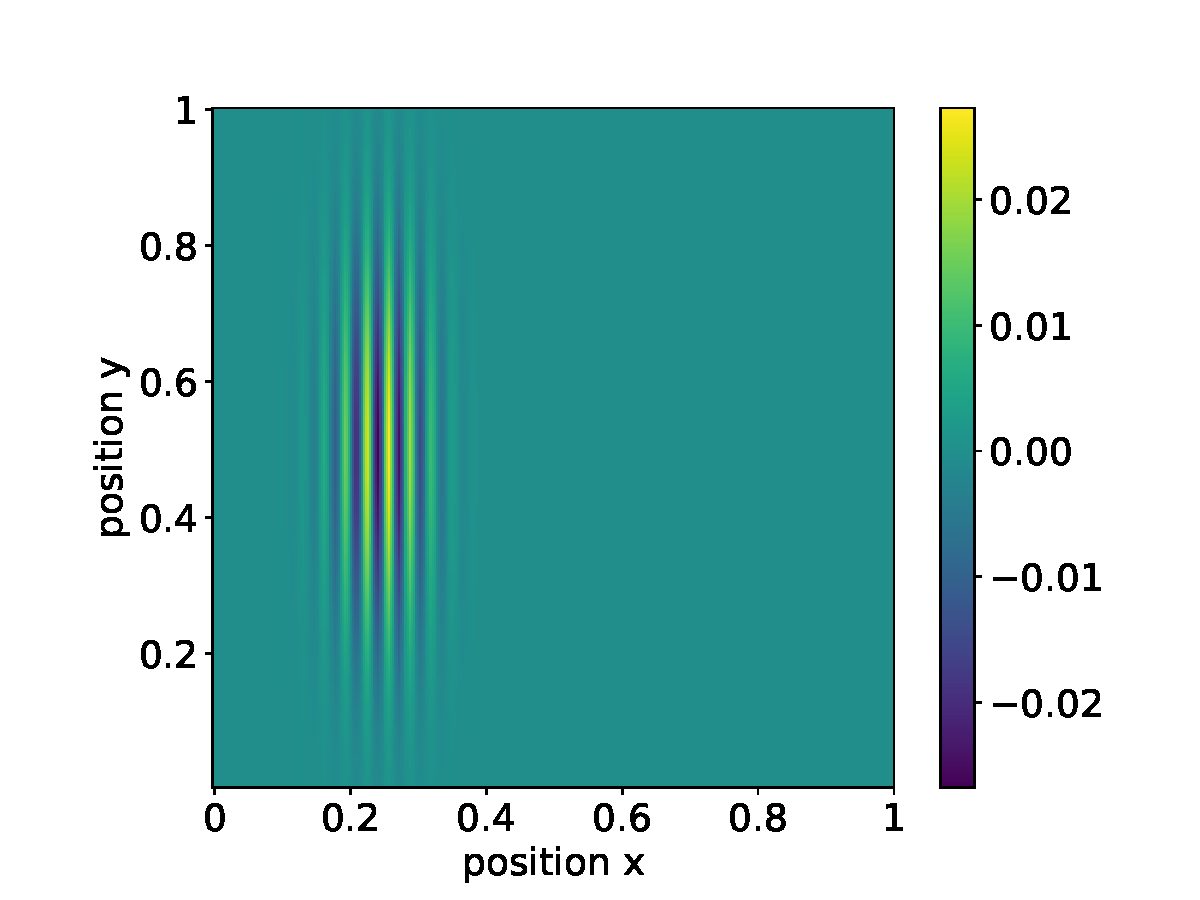
\includegraphics[scale=0.35]{figures/contur_imag_2_t0.pdf} %Imports the figure.
    \caption{Plot showing the imaginary part of the wavefunction at a time $t=0$. The simulation is identical to the one in figure \ref{fig:2}.}
    \label{fig:8}
\end{figure}
\FloatBarrier

\begin{figure}[h!]
    \centering %Centers the figure
    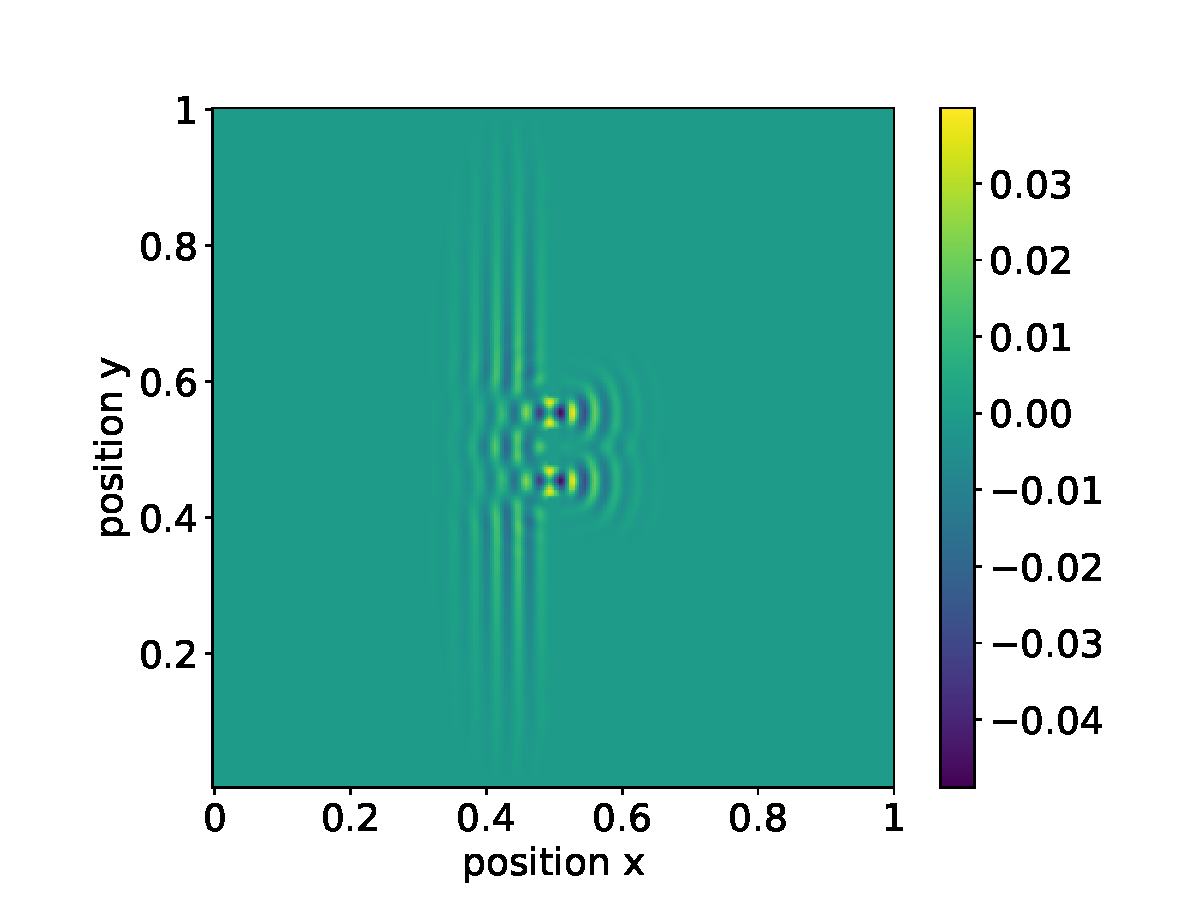
\includegraphics[scale=0.35]{figures/contur_imag_2_12T.pdf} %Imports the figure.
    \caption{Plot showing the imaginary part of the wavefunction at a time $t=0.001$. The simulation is identical to the one in figure \ref{fig:2}.}
\end{figure}
\FloatBarrier

\begin{figure}[h!]
    \centering %Centers the figure
    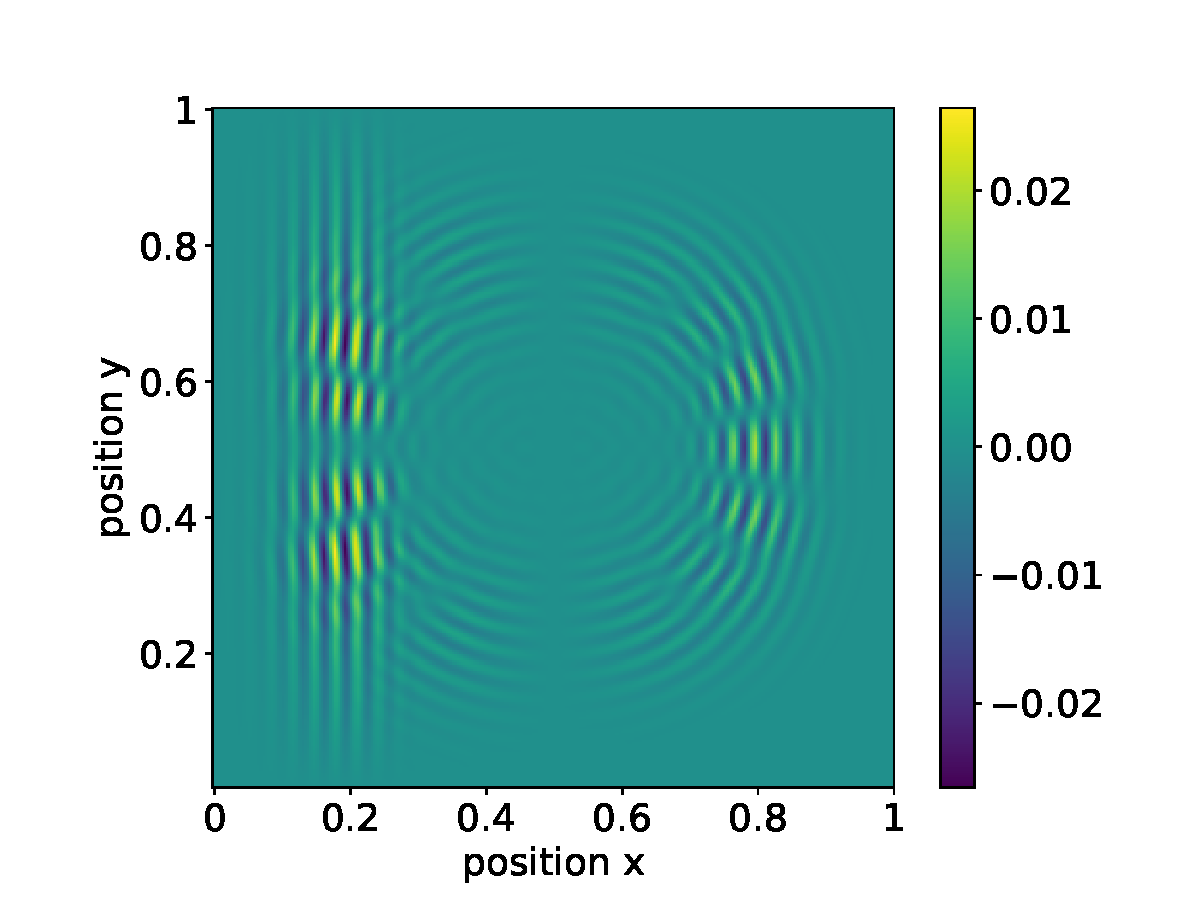
\includegraphics[scale=0.35]{figures/contur_imag_2_T.pdf} %Imports the figure.
    \caption{Plot showing the imaginary part of the wavefunction at a time $t=0.002$. The simulation is identical to the one in figure \ref{fig:2}.}
    \label{fig:10}
\end{figure}
\FloatBarrier

As we can see, the ripples have maintained their orientation along the x-axis. Only the diffraction by the slits seems to have affected their orientation, which is mostly visible for time $t=T$. The ripples are too small to tell with certainty wheater and how much they are phaseshifted, but by the values within the slits at time $t=\frac{1}{2}$, we can at least tell they are not identical. Generally, we can see that both the wave function and the probability densities are almost zero in the wall, which is something we did expect.

Finally, in the last part, we wish to visualize detection probability at a set time, on a screen located behind the slits. Here we will reuse the results from the double slit simulation, and also simulate with single and triple slits. Here we expect to see interference patterns for both double and triple slit, but not for single slit. For the single slit, there might be some diffraction, but as the screen is located close to the slits, in comparison to their size, this might not be visible. Normalized probability mass functions showing this, are in figures \ref{fig:11} to \ref{fig:13}

\begin{figure}[h!]
    \centering %Centers the figure
    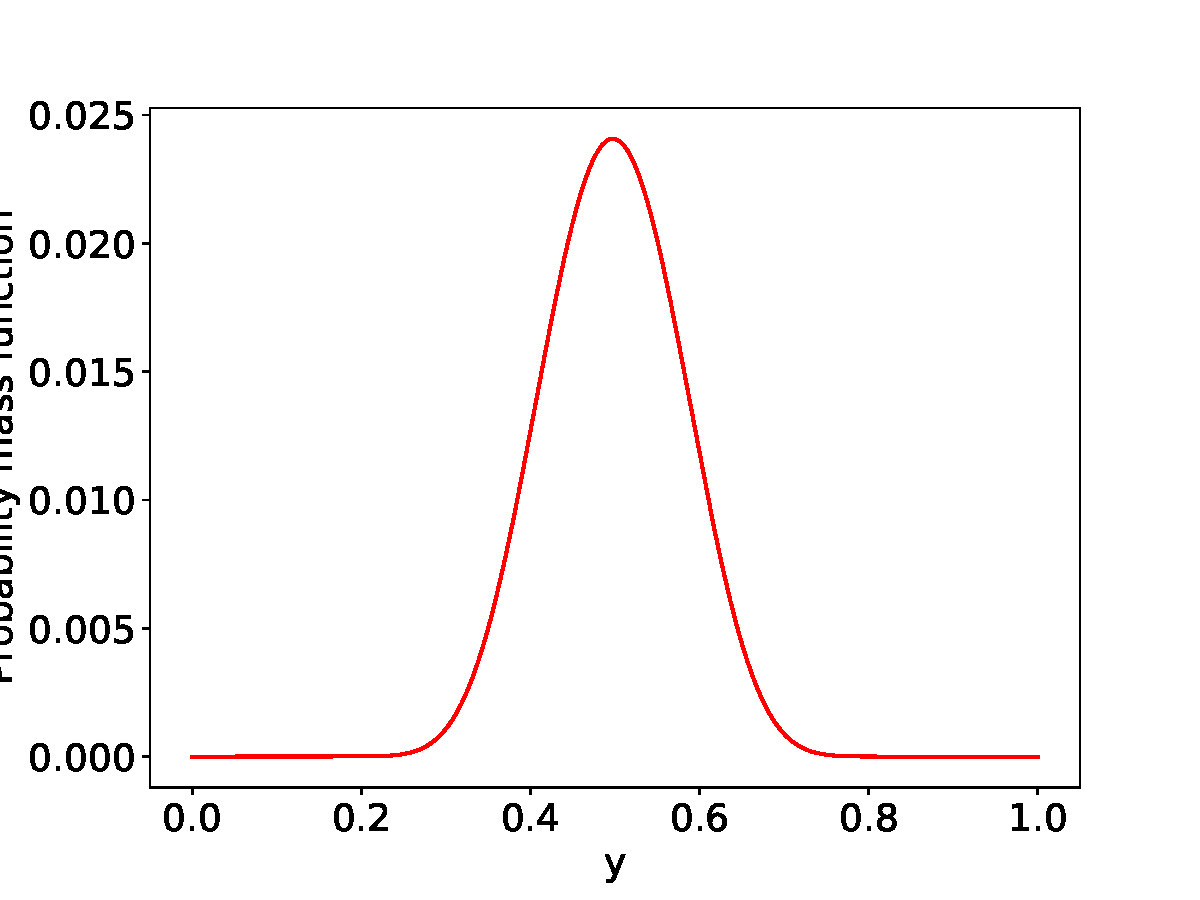
\includegraphics[scale=0.35]{figures/1D_1.pdf} %Imports the figure.
    \caption{Plot showing normalized probability mass function of detection probability at a time $t=0.002$ at a screen, parallel with y-axis located at $x=0.8$ of a single slit. The simulation has identical values, except the number of slits, as the one used for figure \ref{fig:2}.}
    \label{fig:11}
\end{figure}
\FloatBarrier

\begin{figure}[h!]
    \centering %Centers the figure
    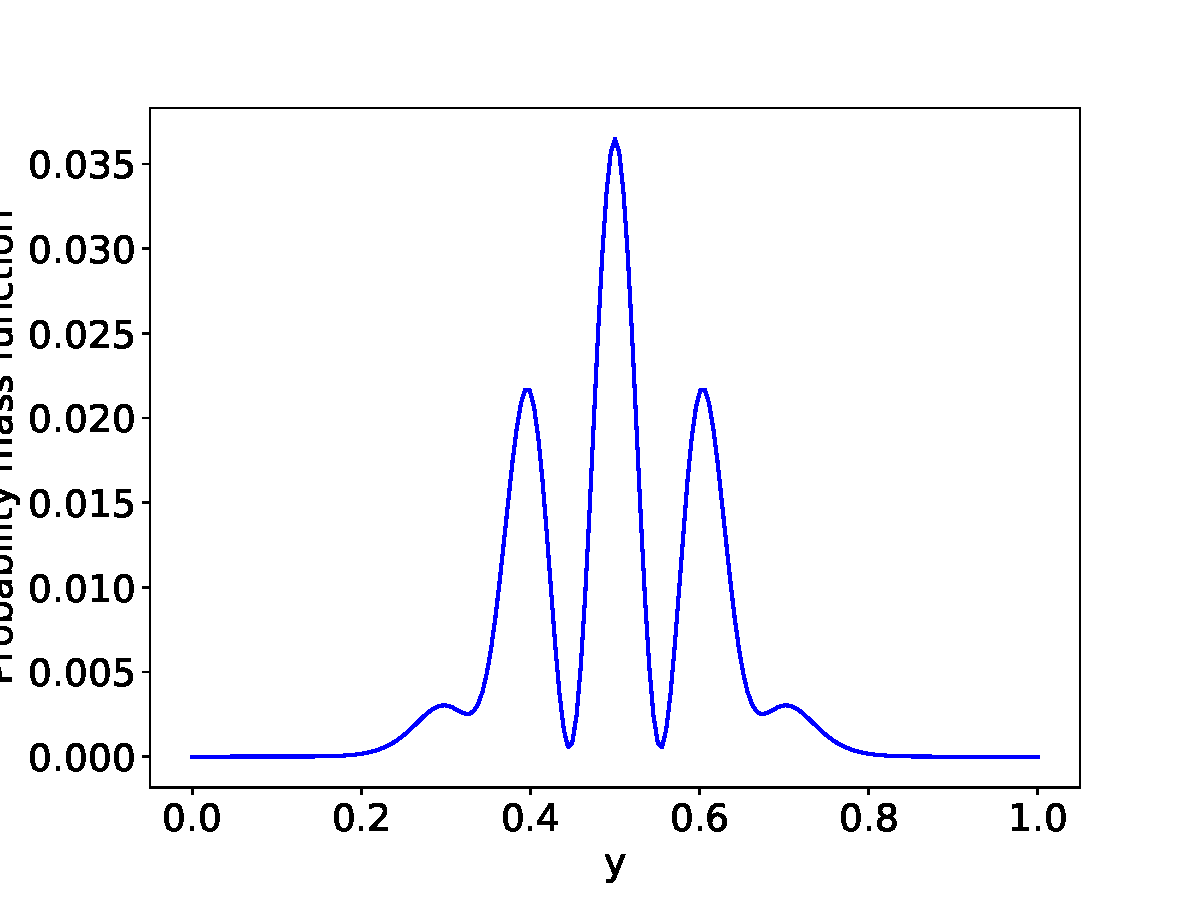
\includegraphics[scale=0.35]{figures/1D_2.pdf} %Imports the figure.
    \caption{Plot showing normalized probability mass function of detection probability at a time $t=0.002$ at a screen, parallel with y-axis located at $x=0.8$ of a double slit. The simulation has identical values, except the number of slits, as the one used for figure \ref{fig:2}.}
    \label{fig:12}
\end{figure}
\FloatBarrier


These functions look as expected. However, again these plots would be more descriptive with probability density, instead of the mass function. It is unreasonable to plot a mass function as a continuous plot, instead of a histogram. In the future, it might be interesting to study the detection probability at a point on the screen at all times. Although not visible from these plots, as they are normalized, it has shown that the probability of particles being detected behind the slits grows with the number of slits, which seems intuitively correct.



\begin{figure}[h!]
    \centering %Centers the figure
    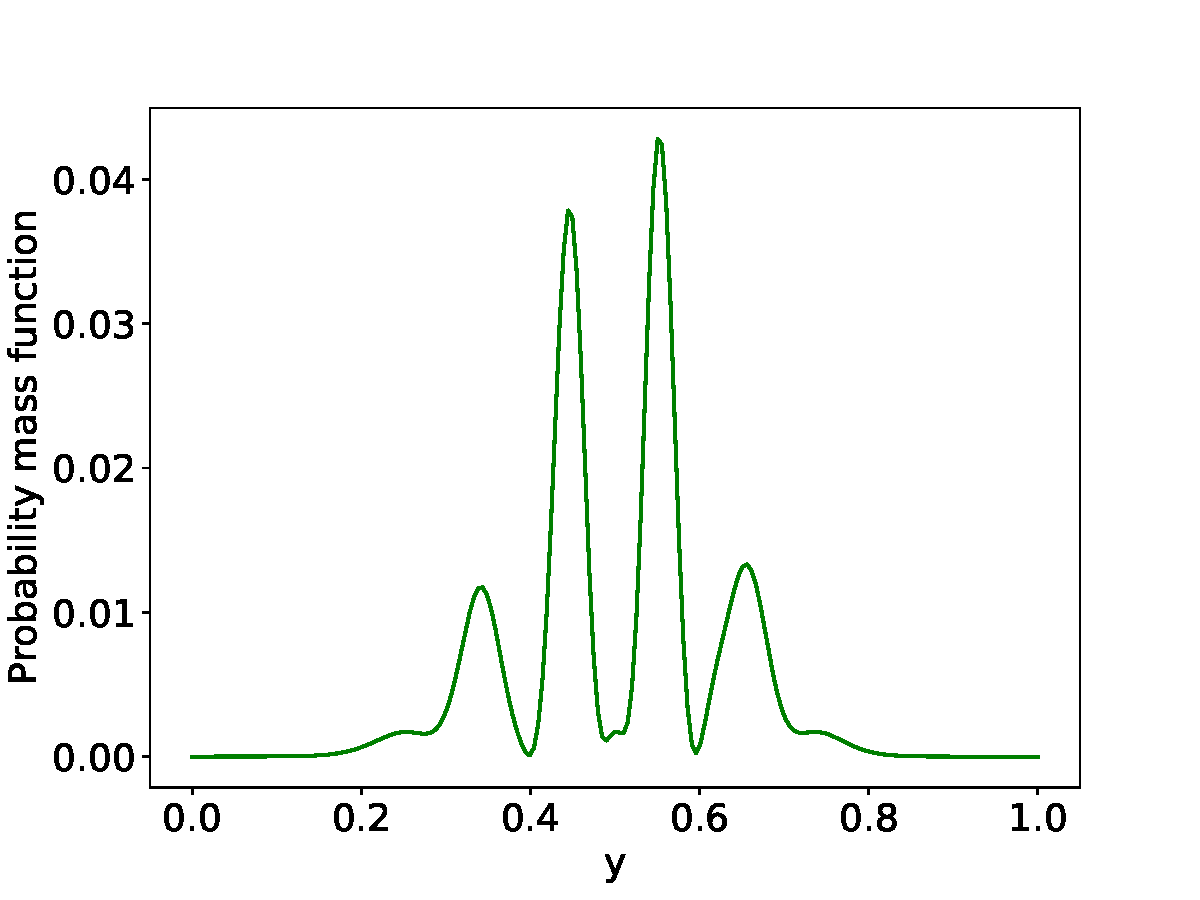
\includegraphics[scale=0.35]{figures/1D_3.pdf} %Imports the figure.
    \caption{Plot showing normalized probability mass function of detection probability at a time $t=0.002$ at a screen, parallel with y-axis located at $x=0.8$ of a triple slit. The simulation has identical values, except the number of slits, as the one used for figure \ref{fig:2}.}
    \label{fig:13}
\end{figure}
\FloatBarrier






% ===========================================
\section{Conclusion}\label{sec:conclusion}

We made a code capable of numerically simulating the evolution of a dimensionless wavefunction in an infinite square well, using the Crank-Nicolson Scheme. The initial wavefunction is a complex wavepacket, which can have different deviations, position, and momenta. We used single, double, and triple slits as barriers for the moving wavepacket and examined its behavior. We have found the probability density creates an interference pattern for both double and triple slits. The ripples in both real and imaginary space of the wavefunction seemed to conserve their orientation unless affected by diffraction from the slits. The probability of detecting a particle behind the slits grew with their number, and some portion of the wavefunction was always reflected.




% ===========================================
\onecolumngrid
% \bibliographystyle{apalike}
\bibliographystyle{unsrt}
\bibliography{ref}


\section{Referances}

GitHub repository containing all code used:
\url{https://github.uio.no/lukasce/FYS3150_Project_5.git}

[1] Timpson, Christopher Gordon (2008). "Quantum Bayesianism: A study" (postscript). Studies in History and Philosophy of Science Part B: Studies in History and Philosophy of Modern Physics. 39 (3): 579–609.

[2] Computational Physics compendium by  Morten Hjorth-Jensen, Department of Physics, University of Oslo




\section{Appendix A}
\subsection{Crank Nicolson Scheme}
CNS uses a linear combination of difference at time $t_n$ and $t_{n+1}$ to represent the room derivatives. Generally, this can be denoted as
$$ \frac{u_{ij}^{n+1} - u_{ij}^n}{\Delta t} =  \theta F_i^{n+1} + (1 - \theta) F_i^{n}. $$
Here $F_{ij}^n$ corresponds to the forward differance at time $t_n$, positions $x_i$, $y_j$ and $theta$ is a number in the interval $[0,1]$. Specifically, for CNS we have $\theta = \frac{1}{2}$, meaning the scheme becomes:
$$ \frac{u_{ij}^{n+1} - u_{ij}^n}{\Delta t} = \frac{1}{2} \Big[ F_i^{n+1} + F_i^{n} \Big]. $$

if we now use the equation \ref{eq:2}, we get

$$ i \frac{u_{ij}^{n+1} - u_{ij}^{n}}{\Delta t} = - \frac{1}{2} \Big[ \frac{u_{i+1j}^{n+1} - 2u_{ij}^{n+1} + u_{i-1j}^{n+1}}{h^2} + \frac{u_{i+1j}^{n} - 2u_{ij}^{n} + u_{i-1j}^{n}}{h^2} \Big] $$
$$ = - \frac{1}{2} \Big[ \frac{u_{ij+1}^{n+1} - 2u_{ij}^{n+1} + u_{ij-1}^{n+1}}{h^2} + \frac{u_{ij+1}^{n} - 2u_{ij}^{n} + u_{ij-1}^{n}}{h^2} \Big] + v_{ij} \frac{1}{2} \Big[u^{n+1}_{ij} + u^{n}_{ij} \Big]. $$


Note that $i$ in an index is an integer, whereas $i$ everywhere else is the imaginary constant. Finally, multiplying the whole equation by $\Delta t/i$, using the fact $\frac{1}{i} = -i$, introducing a new constant $r \equiv \frac{i \Delta t}{2 h^2}$ and collecting all terms at time $t_{n+1}$ at one side of the equation and $t_{n}$ at the second, we get

$$ u_{ij}^{n+1} - r \Big[ \frac{u_{i+1j}^{n+1} - 2u_{ij}^{n+1} + u_{i-1j}^{n+1}}{h^2} \Big] - r \Big[ \frac{u_{ij+1}^{n+1} - 2u_{ij}^{n+1} + u_{ij-1}^{n+1}}{h^2} \Big] + \frac{i \Delta t}{2} v_{ij} u_{ij}^{n+1} $$
$$ = u_{ij}^{n} + r \Big[ \frac{u_{i+1j}^{n} - 2u_{ij}^{n} + u_{i-1j}^{n}}{h^2} \Big]
+ r \Big[ \frac{u_{ij+1}^{n} - 2u_{ij}^{n} + u_{ij-1}^{n}}{h^2} \Big] - \frac{i \Delta t}{2} v_{ij} u_{ij}^{n} . $$


\end{document}
